\chapter{Análisis de intervalos}

El Análisis de Intervalos es una rama de las Matemáticas que lidia con los problemas de redondeo debido al uso de la aritmética de coma flotante. Los ordenadores tienen registros de coma flotante para representar los números reales. Como es bien sabido, hay números reales que no tienen representación finita, por esa razón estos números tienen que ser redondeados.
\\Este tipo de situación crea problemas de imprecisión numérica que se puede propagar y acumular a los largo de los algoritmos, en especial en aquellos que son recursivos.
\\Aunque es posible trabajar con un gran tamaño de bits para representar a los números, este conjunto de números es, de hecho, una representación digital que, obviamente, no tiene las mismas propiedades que el conjunto de números reales.
\\Un ejemplo muy básico puede mostrarnos este problema:
\begin{itemize}
	\item a = \texttt{random()}
	\item b = \texttt{random()}
	\item c = a + b
	\item c = c - a - b
\end{itemize}

Por lógica de cómo trabajamos con el conjunto de números reales se esperaría que el valor final de $c$ sea cero, pero este puede no ser el caso dependiendo del programa de cálculo que tomemos en un ordenador convencional.

Hay una gran cantidad de áreas de investigación en las cuales en Análisis de Intervalos ha sido aplicado para mantener la precisión numérica: Ingeniería de control y supervisión, modelización geométrica y diseño por ordenador.
\\Aparte también hay una serie de{ \em catástrofes} documentadas que podrían haber sido evitadas usando Análisis de Intervalos. Por ejemplo:
\begin{itemize}
	\item Un misil Patriot falló debido a la acumulación de errores de redondeo.
	\item La explosión del Arianne 5 causada por un error de exceso.
\end{itemize}

En este capítulo presentaremos la nociones, operaciones y propiedades básicas del Análisis de Intervalos. Además también haremos una introducción al Análisis de Intervalos Modal que completa la definición clásica de Análisis de Intervalos.

\section{Planteamiento}

La computación numérica de problemas teóricos en un ordenador requiere que los números reales $\mathbb{R}$ sean representados con una cantidad limitada de cifras decimales. Por supuesto, es posible usar un conjunto de números suficientemente grande de números con una gran cantidad de cifras decimales, pero aún así habrá números reales que no podrán ser representados.
\\Esto significa que, cuando traducimos un problema teórico a un problema computacional, estamos trabajando con un conjunto de{ \em números digitales}, llámese $DI$, también conocidos como números en coma flotante.

Los números reales dan soporte a aquellos modelos donde las magnitudes continuas están presentes. Sin embargo, como sabemos, los ordenadores trabajan con truncamiento de números reales. Por tanto, es posible que parte de la información se pierda. Las operaciones deberían restringirse a un intervalo obtenido por medias de redondeo, lo que nos da una identificación operacional de los valores calculados.

Dados dos valores reales $\underline{a}$ y $\overline{a}$, un intervalo $A$ se define como
\begin{equation}
A = [\underline{a},\overline{a}] = \{ x \in \mathbb{R} : \underline{a} \leq x \leq \overline{a} \},
\nonumber
\end{equation}
donde $\underline{a}$ y $\overline{a}$ se conocen como el ínfimo y el supremo del intervalo respectivamente.

Para mantener la representación exacta del número, debemos realizar redondeo al número digital más próximo. Este redondeo es necesario para que la definición anterior sea válida. El uso del Análisis de Intervalos con números digitales nos proporciona un control automático de los errores de redondeo.

En la construcción de intervalos, denotados por $I(\mathbb{R})$, muchas de las propiedades de los números reales se pierden, véase la propiedad distributiva, y se obtienen otras como la relación de inclusión.
\\ Los ordenadores trabajan con el conjunto $DI$, por esa razón el conjunto de intervalos con base en $DI$, denotado por $I(DI)$, es el usado para las operaciones algorítmicas. Esto significa que, mientras $I(DI)$ admita operaciones sobre el conjunto $DI$ para ser tratadas por ordenador, se puede establecer un modelo analítico de operaciones y relaciones de los intervalos análogo al de los intervalos $I(\mathbb{R})$.

Como los intervalos que trataremos a a partir de ahora no son intervalos de números reales significa que los algoritmos que aplicamos a éstos deberán ser modificados para adaptarse a la nueva aritmética.

\section{Relaciones entre intervalos}

Las relaciones entre los intervalos son equivalentes a algunas relaciones entre los límites del intervalo. Aunque la definición de las relaciones a veces no son evidentes, hay una norma general de tomar la definición más útil en cada caso. Lo importante es obtener relaciones parecidas a los intervalos de números reales.

\begin{definition}
Se dice que dos intervalos $A$ y $B$ son iguales, denotado por $A = B$, si para todo $a \in A$ existe $b \in B$ tal que $a = b$ y viceversa. En función de los límites:
$$A = B \iff \underline{a} = \underline{b} \text{ y } \overline{a} = \overline{b}.$$
\end{definition}

\begin{definition}
Se dice que dados dos intervalos, $A$ y $B$, $A < B$ si para todo $a \in A$ y $b \in B$ se tiene que $a < b$. En función de los límites:
$$A < B \hbox{ si y sólo si } \overline{a} < \underline{b}.$$
\end{definition}

\begin{definition}
Se dice que dados dos intervalos, $A$ y $B$, $A \leq B$ si para todo $a \in A$ existe $b \in B$ tal que $a \leq b$ y para todo $b \in B$ existe $a \in A$ tal que $a \leq b$. En función de los límites:
$$A \leq B \iff \underline{a} \leq \underline{b} \hspace{0.25cm} \text{y} \hspace{0.25cm} \overline{a} \leq \overline{b}.$$
\end{definition}

\begin{definition}
Se dice que dados dos intervalos, $A$ y $B$, $A \subset B$ si para todo $a \in A$ se tiene que $a \in B$. En función de los límites:
$$A \subset B \iff \underline{a} \geq \underline{b} \hspace{0.25cm} \text{y} \hspace{0.25cm} \overline{a} \leq \overline{b}.$$
\end{definition}

\begin{definition}
Se dice que dados dos intervalos, $A$ y $B$, $A$ es incidente en $B$, $A =_{\nparallel} B$, si $A \cap B \neq \emptyset$. En función de los límites:
$$A =_{\nparallel} B \iff \max(\underline{a},\underline{b}) \leq \min(\overline{a},\overline{b}).$$
\end{definition}

\section{Operaciones de Aritmética de Intervalos}

Las operaciones de los intervalos se basan en la Teoría de Conjuntos. De esta manera es posible definir las operaciones mediante medias de los límites de los intervalos.


Hay ciertas condiciones que deben cumplir las operaciones:
\begin{itemize}
	\item El resultado de una operación entre intervalos ha de ser otro intervalo.
	\item La restricción de una operación de intervalos entre dos intervalos particulares debe coincidir con la misma operación realizada entre intervalos reales.
	\item Todas las operaciones entre elementos particulares de ambos intervalos deben de estar contenidas en el intervalo final. Esto es conocido como el Principio de Inclusión.
\end{itemize}
De acuerdo a estas condiciones, las operaciones se definen por la expresión
\begin{equation}
AwB = \{ awb : a \in A, b \in B \},
\end{equation}
donde $w$ representa cualquiera de las operaciones.

La ecuación general de las operaciones de Aritmética de Intervalos es
\begin{equation}
AwB = [ \min(\underline{a}w\underline{b},\underline{a}w\overline{b},\overline{a}w\underline{b},\overline{a}w\overline{b}), \max(\underline{a}w\underline{b},\underline{a}w\overline{b},\overline{a}w\underline{b},\overline{a}w\overline{b}) ]
\nonumber
\end{equation}

Por tanto, las cuatro operaciones básicas se definen como
\begin{equation}
\begin{tabular}{l}
$[\underline{a},\overline{a}] + [\underline{b},\overline{b}] = [\underline{a} + \underline{b},\overline{a} + \overline{b}]$, \\
$[\underline{a},\overline{a}] - [\underline{b},\overline{b}] = [\underline{a} - \overline{b},\overline{a} - \underline{b}]$, \\
$[\underline{a},\overline{a}] * [\underline{b},\overline{b}] = [min(\underline{a}\underline{b},\underline{a}\overline{b},\overline{a}\underline{b},\overline{a}\overline{b}), \max(\underline{a}\underline{b},\underline{a}\overline{b},\overline{a}\underline{b},\overline{a}\overline{b})]$, \\
$[\underline{a},\overline{a}] / [\underline{b},\overline{b}] = [\underline{a},\overline{a}]*[\frac{1}{\overline{b}},\frac{1}{\underline{b}}] \text{ si } 0 \notin [\underline{b},\overline{b}]$.
\end{tabular}
\nonumber
\end{equation}

\section{Intervalos modales}

El Análisis de Intervalos Modales, MIA por sus siglas en inglés, es un complemento lógico del Análisis de Intervalos clásico que incluye herramientas para resolver incertidumbre cuantificada. Para alcanzar este objetivo, la versión clásica se asocia con un cuantificador.

Un intervalo modal se define como un par $(I,Q)$ donde $I$ es un intervalo clásico y $Q$ es un cuantificador modal, véase $\forall$ o $\exists$ llamados universal y existencial, respectivamente. El conjunto de intervalos modales se representa por $I^*(\mathbb{R})$. Si el intervalo modal se asocia con un cuantificador existencial se llama{ \em propio} y en caso de que esté asociado con un cuantificador universal se llama{ \em impropio}. La representación canónica de un intervalo modal es:
\begin{itemize}
	\item Intervalo propio: $X = [a,b] = ([a,b]',\exists)$ si $a \leq b$.
	\item Intervalo impropio: $X = [a,b] = ([b,a]',\forall)$ si $a \geq b$.
	\item Intervalo puntual: $X = [a,b] = ([a,b]',\{ \exists, \forall \})$ si $a = b$.
\end{itemize}
Donde la notación $'$ indica un intervalo clásico.

\begin{remark}
Un intervalo puntual puede ser considerado tanto propio como impropio.
\end{remark}

El proceso de construcción de intervalos modales se completa con el concepto de cuantificador modal $Q$ definido por
\begin{equation}
Q(x,X)P(x) := \left\{ \begin{tabular}{l l l}
$(\exists x \in X')P(x)$ & & $X = (X', \exists)$, \\
& & \\
$(\forall x \in X')P(x)$ & & $X = (X', \forall)$,
\end{tabular}
\right.
\nonumber
\end{equation}
donde $P(x)$ es un predicado con variable libre $x$. Esto define el conjunto de predicados reales aceptados por un intervalo modal $A = (A',Q_A)$ como
\begin{equation}
Pred((A',Q_A)) := \{ P(.) \in Pred(\mathbb{R}) : Q(x,(A',Q_A))P(x) \}.
\nonumber
\end{equation}
donde $ Pred(\mathbb{R})$ es el conjunto de predicados con variable real.

Esta definición del cuantificador modal $Q$ nos obliga a introducir un cambio en la notación clásica para los cuantificadores. En lo sucesivo usaremos:
\begin{itemize}
\item $\exists(x,X')$ en lugar de $\exists x \in X'$.
\item $\forall(x,X')$ en lugar de $\forall x \in X'$.
\end{itemize}

A través de la identificación de un intervalo modal con el conjunto de tales predicados reales en los que aceptamos $X \iff P(X)$, surge la inclusión de dos intervalos como la inclusión del conjunto de predicados que aceptan, esto es, si $X, Y  \in I^*(\mathbb{R})$ se tiene
\begin{equation}
X \subset Y \iff Pred(X) \subset Pred(Y).
\nonumber
\end{equation}

Usando las coordenadas canónicas $X = [x_1,x_2]$ e $Y = [y_1,y_2]$ esta inclusión mantiene el mismo{ \em modus operandi} tradicional, esto es,
\begin{equation}
[x_1,x_2] \subset [y_1,y_2] \iff y_1 \leq x_1 \hspace{0.25cm} \text{y} \hspace{0.25cm} x_2 \leq y_2.
\nonumber
\end{equation}

La siguiente figura nos muestra la representación geométrica de los intervalos modales y la relación de inclusión.
\begin{figure}[h]
\centering
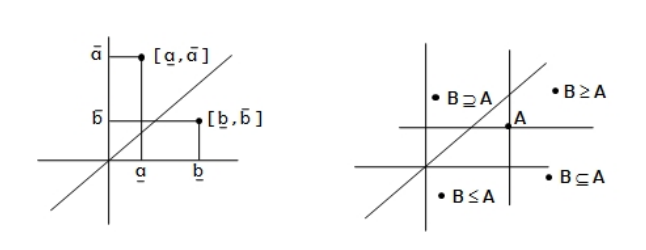
\includegraphics[scale=0.5]{images/florez11.png}
\caption{La primera imagen nos muestra la representación de los intervalos modales y la segunda las inclusiones y las desigualdades.}
\end{figure}

\newpage
Las operaciones{ \em meet} y{ \em join} en $I^*(\mathbb{R})$ para una familia acotada de intervalos modales $A(I) := \{ A(i) = [a_1(i),a_2(i)] \in I^*(\mathbb{R}) : i \in I \}$, donde $I$ es el el dominio de índices, se definen por
\begin{equation}
\wedge(i,I) A(i) = A \in I^*(\mathbb{R}) \text{ es  tal que } \forall (i,I) X \subset A(i) \iff X \subset A,
\nonumber
\end{equation}
\begin{equation}
\vee(i,I) A(i) = B \in I^*(\mathbb{R}) \text{ es  tal que } \forall (i,I) X \supset A(i) \iff X \supset B.
\nonumber
\end{equation}
notado como $(A \wedge B)$ y $(A \vee B)$ para el caso correspondiente. El resultado, visto como función de los límites de los intervalos, es
\begin{equation}
\bigwedge_{i \in I} A(i) = [\max_{i \in I} a_1(i), \min_{i \in I} a_2(i)],
\nonumber
\end{equation}
\begin{equation}
\bigvee_{i \in I} A(i) = [\min_{i \in I} a_1(i), \max_{i \in I} a_2(i)].
\nonumber
\end{equation}

Con estas operaciones el conjunto de intervalos modales es un retículo para la $\subset$-relación, mientras que los intervalos clásicos no lo son, por tanto, estamos completando el conjunto de los intervalos clásicos.

Ambos operadores son isotónicos, i.e.,  si $A_i \subset B_i$ para cada $i \in I$, entonces
\begin{equation}
\bigwedge_{i \in I} A_i \subset \bigwedge_{i \in I} B_i,
\nonumber
\end{equation}
\begin{equation}
\bigvee_{i \in I} A_i \subset \bigvee_{i \in I} B_i.
\nonumber
\end{equation}

En el conjunto de los números conocemos que hay dos relaciones $\leq$ y $\geq$, y las extensiones de estas relaciones a los intervalos se definen por
\begin{equation}
[x_1,x_2] \leq [y_1,y_2] \iff x_i \leq y_i \hspace{0.5cm} i = 1,2.
\nonumber
\end{equation}
Lo que nos conduce a los operadores $\min$ y $\max$ para una familia acotada de intervalos modales $A(I) := \{ A(i) \in I^*(\mathbb{R}) : i \in I \}$ como:
\begin{equation}
\min_{i \in I} A(i) = A \in I^*(\mathbb{R}) \text{ es  tal que } \forall (i,I) X \leq A(i) \iff X \leq A
\nonumber
\end{equation}
\begin{equation}
\max_{i \in I} A(i) = B \in I^*(\mathbb{R}) \text{ es  tal que } \forall (i,I) X \geq A(i) \iff X \geq B
\nonumber
\end{equation}
Computacionalmente expresado:
\begin{equation}
\min_{i \in I} A(i) = [\min_{i \in I} a_1(i), \min_{i \in I} a_2(i)]
\nonumber
\end{equation}
\begin{equation}
\max_{i \in I} A(i) = [\max_{i \in I} a_1(i), \max_{i \in I} a_2(i)]
\nonumber
\end{equation}

El conjunto de los intervalos modales es, por tanto, un retículo bajo la $\leq$-relación. La siguiente figura nos muestra la representación geométrica de los operadores que hemos definido para dos intervalos.
\begin{figure}[h]
\centering
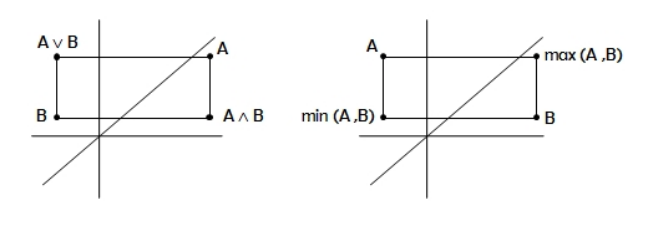
\includegraphics[scale=0.5]{images/florez12.png}
\end{figure}

\subsection{Extensiones semánticas}

En la teoría clásica de Análisis de Intervalos una extensión de una función de $\mathbb{R}^n$ a $\mathbb{R}$ dada por $z = f(x_1, \dotso, x_n)$ es el intervalo de extensión unida $R_f$ de $f$. Para el intervalo $X' = (X_1',\dotso, X_n') \in I(\mathbb{R}^n)$ se define el rango de $f$-valores en $X'$ como
\begin{equation}
R_f(X_1',\dotso, X_n') := \{ f(x_1, \dotso, x_n) : x_i \in X_i' \ \forall i \in \{1, \dotso, n \} \} =
\nonumber
\end{equation}
\begin{equation}
[\min \{ f(x_1, \dotso, x_n) : x_i \in X_i' \ \forall i \in \{1, \dotso, n \} \}, \max \{ f(x_1, \dotso, x_n) : x_i \in X_i' \ \forall i \in \{1, \dotso, n \} \}].
\nonumber
\end{equation}

Para obtener la estimación para la extensión unida, las extensiones racionales del intervalo teórico $fR(X_1', \dotso, X_n')$ se definen como su correspondiente función real-racional $f(x_1, \dotso, x_n)$ reemplazando:
\begin{enumerate}
\item Los argumentos numéricos $x_i$ por sus argumentos de intervalos $X_i'$.
\item Los operadores aritméticos{ \em reales} $\omega$ por su correspondiente operación entre intervalos la cual, en los casos más comunes de computaciones truncadas de cualquier aritmética tiene que dirigirse al exterior $\omega^R$ debido a la inclusión
$$X' \omega Y' \subset X' \omega^R Y' := Out(X' \omega Y'),$$
donde $Out$ representa el redondeo exterior del intervalo $X' \omega Y'$.
\end{enumerate}

Las funciones de intervalos racionales tienen la propiedad, fundamental para todo el cuerpo de Análisis de Intervalos, de ser inclusiva, esto es, para un conjunto de intervalos cumpliendo $X_1' \subset Y_1', \dotso, X_n' \subset Y_n'$ se cumple
\begin{equation}
f R(X_1', \dotso, X_n') \subset f R(Y_1', \dotso, Y_n').
\nonumber
\end{equation}
Suponiendo que no ocurre  ninguna división entre un intervalo que contenga al cero.

La relación entre ambas extensiones es
\begin{equation}
R_f(X_1', \dotso, X_n') \subset f R(X_1', \dotso, X_n').
\nonumber
\end{equation}
Donde $f R$ es computable a parir de los límites de los intervalos $X_1', \dotso, X_n'$ y normalmente representan una sobrestimación de $R_f(X_1', \dotso, X_n')$.

En el Análisis de Intervalos Modales, un rol similar al de $R_f$ se ve cubierto de forma semántica por las funciones * y **, denotadas por $f^*$ y $f^{**}$ (funciones estrella y doble estrella) y definidas por:
\begin{equation}
f^*(X) := \bigvee_{x_p \in X_p'} \bigwedge_{x_i \in X_i'} [f(x_p,x_i),f(x_p,x_i)] = \left[ \min_{x_p \in X_p'} \max_{x_i \in X_i'} f(x_p,x_i), \max_{x_p \in X_p'} \min_{x_i \in X_i'} f(x_p,x_i) \right]
\nonumber
\end{equation}
\begin{equation}
f^{**}(X) := \bigwedge_{x_i \in X_i'} \bigvee_{x_p \in X_p'} [f(x_p,x_i),f(x_p,x_i)] = \left[ \max_{x_p \in X_p'} \min_{x_i \in X_i'} f(x_p,x_i), \min_{x_p \in X_p'} \max_{x_i \in X_i'} f(x_p,x_i) \right]
\nonumber
\end{equation}
Las cuales tienen, por supuesto, la propiedad de inclusión $f^*(X) \subset f^{**}(X)$. Además
\begin{equation}
X \subset Y \Rightarrow f^*(X) \subset f^*(Y) \ \text{ y } \ f^{**}(X) \subset f^{**}(Y).
\nonumber
\end{equation}
En algunos casos puede ocurrir que $f^* \equiv f^{**}$.

Los próximos teoremas nos dan una interpretación lógica de las extensiones semánticas.

\begin{theorem}{\textbf{Teorema de la semántica *:}}\label{theorem1}
Sea $X \in I^*(\mathbb{R}^n)$ y $Z \in I^*(,\mathbb{R})$, se tiene
$$f^*(X) \subset Z \iff \forall(x_p, X_p') \ Q(z,Z) \ \exists (x_i,X_i') \ z = f(x_p,x_i).$$
\end{theorem}

\begin{theorem}{\textbf{Teorema de la semántica **:}}\label{theorem2}
Sea $X \in I^*(\mathbb{R}^n)$ y $Z \in I^*(,\mathbb{R})$, se tiene
$$f^*(X) \supset Z \iff \forall(x_i, X_i') \ Q(z,Dual(Z)) \ \exists (x_p,X_p') \ z = f(x_p,x_i).$$
\end{theorem}

Esto significa que es posible reducir una expresión lógica a inclusiones entre intervalos. Ambos teoremas hacen equivalente una fórmula lógica, con intervalos y predicados funcionales donde los cuantificadores universales preceden a los existenciales, a una inclusión de intervalos.

Por ejemplo, la función real $f(x,y) = x+y$ con los intervalos $X = [1,3]$ e $Y = [2,3]$ el resultado es $X + Y = [4,5]$. De acuerdo al teorema de la semántica * obtenemos
$$\forall(x,[1,3]')\exists(z,[4,5]')\exists(y,[2,3]')x+y=z.$$
Y de acuerdo al teorema de la semántica ** obtenemos
$$\forall(y,[2,3]')\exists(z,[4,5]')\exists(x,[1,3]')x+y=z.$$

Incluso pensando que las funciones $f^*$ y $f^{**}$ son óptimas en el sentido semántico, estos teoremas no explicitan el proceso de computación del intervalo $Z$ que verifica $f^* \subset Z$ ó $f^{**} \supset Z$, i.e., intervalos que son una estimación exterior e interior de $f^*$ y $f^{**}$ respectivamente. De hecho, exceptuando los operadores aritméticos, el cálculo de $f^*$ y $f^{**}$  no se puede lograr mediante computación directa. Si la función continua $f$ es una función racional, entonces existe  una extensión modal racional que se obtiene usando el programa computacional definido por el árbol sintáctico de las expresiones de la función:

\begin{itemize}
\item Si $f$ es una función racional de $\mathbb{R}^n$ a $\mathbb{R}$, entonces su extensión modal racional a los intervalos modales $X_1, \dotso, X_n$ representada por $f \ R(X_1, \dotso, X_n)$ es la función $f \ R$ de $I^*(\mathbb{R}^n)$ a $I^*(\mathbb{R})$ definida por el programa computacional indicado por la sintaxis de $f$ cuando el operador ral se transforma en su extensión semántica.
\end{itemize}

Las funciones de intervalos modales racionales no son interpretables, pero tiene la propiedad de ser isotónicas, i. e., para intervalos $X_1 \subset Y_1, \dotso, X_n \subset Y_n$ se verifica la relación
\begin{equation}
f \ R(X_1, \dotso, X_n) \subset f \ R(Y_1, \dotso, Y_n).
\nonumber
\end{equation}
Asumiendo que no se producen divisiones por intervalos que contengan al cero.

\subsection{Interpretabilidad y optimalidad}

La solución al problema de computar las extensiones semánticas $f^*$ y $f^{**}$ consiste en relacionarlo mediante relaciones de inclusión a algunas extensiones racionales. Las computaciones con $f \ R(X)$ deben de hacerse con truncación externa de cada operador para obtener $f^*(X) \subset f \ R(X)$ y con la truncación interna obtenemos $f \ R(X) \subset f^{**}(X)$. En muchos de los casos la extensión racional $f \ R(X)$ es óptima, i. e.,
\begin{equation}
f^*(X) = f \ R(X) = f^{**}(X).
\nonumber
\end{equation}
Y, exceptuando el redondeo, ambos teoremas semánticos son aplicables al intervalo $f \ R(X)$ proporcionándole un significado lógico a éste.

El Análisis de Intervalos Modales nos proporciona una serie de resultados sobre inclusiones o igualdades que resuelven parte del problema doble de interpretabilidad de extensiones modales racionales y computabilidad de las expresiones semánticas. Ahora mostraremos varios teoremas que nos muestran resultados sobre la interpretabilidad de extensiones racionales.

\begin{theorem}{\textbf{* interpretabilidad de funciones modales racionales:}}\label{th1}
Si las componentes impropias de $X$ son uni-incidentes en $f \ R(X)$ y si $Out(f \ R(Prop(X)))$ existe, entonces
$$Out(f \ R(X)) \supset f^*(X).$$
Donde $Out$ representa el redondeo exterior del intervalo $f \ R(X)$.
\end{theorem}

\begin{theorem}{\textbf{** interpretabilidad de las funciones modales racionales:}}\label{th2}
Si las componentes propias de $X$ son uni-incidentes en $f R(X)$ y si $Out(f \ R(Prop(X)))$, entonces
$$Inn(f \ R(X)) \subset f^{**}(X).$$
Donde $Inn$ representa el redondeo interno del intervalo $f \ R(X)$.
\end{theorem}

Una función real $f$ se llama $x$-totalmente monótona para una variable multi-incidente $x \in \mathbb{R}$ si es uniformemente monótona para esta variable y para cada una de sus incidencias, consideradas como variables independientes.

\begin{theorem}{\textbf{* interpretabilidad con monotonía total:}}\label{th3}
Sea $X$ un vector intervalo y $f \ R$ definido en $Prop(X)$ y totalmente monótona para un subconjunto $Z$ de componentes multi-incidentes. Sea $X \ Dt^*$ el vector agrandado de $X$, esto es, cada incidencia de cada componente multi-incidente del subconjunto con monotonía total está incluida en $X \ Dt^*$ como una componente independiente, pero transformada en su dual si el correspondiente punto incidente tiene un sentido monótono contrario al global de la correspondiente componente $Z$. Para el resto, las componentes impropias muti-indicentes se transforman en un intervalo puntual definido por cualquiera de sus puntos. Entonces
$$f^*(X) \subset f \ R(X \ Dt^*).$$
\end{theorem}

\begin{theorem}{\textbf{** interpretabilidad con monotonía total:}}\label{th4}
Sea $X$ un vector intervalo y $f \ R$ definido en $Prop(X)$ y totalmente monótona para un subconjunto $Z$ de componentes multi-incidentes. Sea $X \ Dt^{**}$ el vector agrandado de $X$, esto es, cada incidencia de cada componente multi-incidente del subconjunto con monotonía total está incluida en $X \ Dt^{**}$ como una componente independiente, pero transformada en su dual si el correspondiente punto incidente tiene un sentido monótono contrario al global de la correspondiente componente $Z$. Para el resto, las componentes propias muti-indicentes se transforman en un intervalo puntual definido por cualquiera de sus puntos. Entonces
$$f^{**}(X) \supset f \ R(X \ Dt^{**}).$$
\end{theorem}

\begin{theorem}{\textbf{Interpretabilidad en el caso general multi-incidente:}}\label{th5}
Si $f \ R(X)$ tiene componentes multi-incidentes impropias y $Xt^*$ se obtiene reemplazando tales componentes por intervalos puntual definido por cualesquiera de sus puntos  de sus dominios, entonces
$$f^*(X) \subset f \ R(X \ t^*).$$
\end{theorem}

Este teorema es útil cuando no es posible realizar test de monotonía.

Es posible obtener mejores resultados si se aplica el concepto de optimalidad.

\begin{definition}
Una función modal racional $f \ R(X)$ se dice óptima si cualquiera de sus operadores no uniformemente monótonos es seguido por operadores de una única variable.
\end{definition}

\begin{theorem}{\textbf{Coerción a la optimalidad:}}\label{th6}
Sean $X$, $f \ R$ y $X \ D$ definidos bajo las condiciones de los teoremas \ref{th3} y \ref{th4}. Y sea $f \ R$ óptimo en $Prop(X)$. En tal caso
$$f^*(X) = f \ R(X \ D) = f^{**}(X).$$
\end{theorem}

Este teorema es útil para resolver el problema, especialmente en el caso cuando la función de la fórmula lógica verifica las condiciones de optimalidad ya que, en este caso, la computación de $f \ R(X \ D)$ es igual a $f^*(X)$, excepto por el redondeo, y el teorema \ref{theorem1} lo hace equivalente a la fórmula lógica.

\textbf{Ejemplo:}

Consideremos una función continua $f : \mathbb{R^2} \to \mathbb{R}$ definida por
$$f(x,y) = \frac{xy}{x+y},$$
con $X = [2,3]$ e $Y = [4,3]$.

La función $f$ es totalmente monótona respecto de $x$ y de $y$ ya que sus derivadas parciales son mayores que cero en los dominios de las variables. Tomando las componentes multi-incidentes como componentes independientes, es decir,
$$f(x_1,x_2,y_1,y_2) = \frac{x_1 y_1}{x_2 + y_2},$$
se tiene que:
$$\frac{\partial f}{\partial x_1} > 0, \hspace{0.5cm} \frac{\partial f}{\partial x_2} < 0, \hspace{0.5cm} \frac{\partial f}{\partial y_1} > 0 \hspace{0.5cm} \text{y} \hspace{0.5cm} \frac{\partial f}{\partial y_2} > 0.$$

Con estas condiciones mostraremos las aplicaciones de tres teoremas:
\begin{enumerate}
\item De acuerdo al teorema \ref{th5} las componentes impropias multi-incidentes se reemplazan por intervalos puntual, $Xt^* = ([2,3],[4,4],[2,3],[4,4])$ el resultado es
$$f \ R(Xt^*) = \frac{X \ [4,4]}{X + [4,4]} = [1.1428,2].$$
\item De acuerdo al teorema \ref{th3} tenemos $X \ Dt^* = ([2,3],[4,4],[3,2],[4,4])$ y el resultado es
$$f \ R(X \ Dt^*) = \frac{X \ [4,4]}{Dual(X) + [4,4]} = [1.3333,1.7144].$$
\item De acuerdo al teorema \ref{th6} tenemos $X \ D = ([2,3],[4,3],[3,2],[3,4])$ y el resultado es
$$f^*(X) = \frac{X Y}{Dual(X) + Dual(Y)} = [1.3333,1.5].$$
\end{enumerate}

La mejor aproximación se obtiene mediante el teorema \ref{th6}. En el lado contrario tenemos la aproximación obtenida mediante el teorema \ref{th5}. En este ejemplo es
$$f^*(X) \subset f \ R(X \ Dt^*) \subset f \ R(Xt^*).$$

\section{Conclusiones}

En este capítulo hemos definido e introducido las diferentes propiedades del Análisis de Intervalos. Como hemos explicado, la Aritmética de Intervalos se puede aplicar a diversos campos de investigación para solucionar los problemas de redondeo. Por supuesto las gráficas por ordenador no iban a ser una excepción.

También hay una visión del Análisis de Intervalos Modales, que completa la definición clásica de Análisis de Intervalos mediante aplicación de los cuantificadores a la definición de intervalo. La teoría de Intervalos Modales nos da los intervalos impropios que en la teoría clásica carece de sentido y, en la mayoría de casos, la transformación lleva tal intervalo impropio en uno propio sin explicación lógica. El Análisis de Intervalos Modales nos concede una explicación para tales casos por medio de las aplicaciones de los teoremas incluidos en este capítulo.

Los teoremas desarrollados son la base para la teoría de Intervalos Modales y, además, nos ayudarán a mejorar el Ray Tracing, o trazado, de superficies implícitas.